\section{Ziel des Versuchs}
In den Versuch sollen ein Reflexklystron und Mikrowellen in einem Hohlleiter untersucht und vermessen werden.
\section{Theorie}
\label{sec:Theorie}
\nocite{skript}
Der Begriff Mikrowellen ist nicht wirklich scharf definiert. Im Allgemeinen wird damit der Frequenzbereich von $\SI{300}{\mega\hertz}$ bis $\SI{300}{\giga\hertz}$ verstanden. Überschneidungen zum Bereich der Radiowellen sind dabei nicht auszuschließen.
\subsection{Hohlleiter}
Ein Hohlleiter ist ein metallisches Rohr, in dem elektromagnetische Wellen geleitet werden. Die Rohre haben meist einen rechteckigen oder runden Querschnitt mit einer gut leitenden Oberflächer auf der Innenseite.
In geeigneten Frequenzen, lassen sich durch Hohlleiter elektrische Signale viel verlustärmer übertragen als in Festkörpern.
In dem Rohr bilden sich stehende Wellen aus, sodass dieses zu einem Hohlraumresonator wird. Wenn in diesem die Maxwellgleichungen gelöst werden, ergibt sich, aufgrund der Randbedingungen, durch die geometrischen Gegebenheiten, eine untere Grenzfrequenz unterhalb dieser sich keine stehende Welle ausbreiten kann.
Bei den Moden der elektromagnetischen Welle wird zwischen transversal magnetischen (TM) und transversal elektrischen (TE) Moden unterschieden. Das bedeutet, dass entweder das magnetische oder das elektrische Feld nur senkrecht zur Ausbreitungsrichtung der Welle schwingen.
\subsection{Das Reflexklystron}
Ein Klystron kann allgemein zur Verstärkung und zur Frequenzmodulation von elektromagnetischen Signalen verwendet werden. In diesem Fall dient ein Reflexklystron als Mikrowellengenerator. Wie in Abb. \ref{fig:kly} zu sehen, werden Elektronen zwischen der Austrittskathode und dem Reflektor hin und her beschleunigt, sodass dieser zu einem Oszillator wird. Die bewegten Ladungen erzeugen, durch das Prinzip der Influenz, im Hohlraumresonator ein elektromagnetisches Feld, welches weitergeleitet und zu weiteren Zwecken verwendet werden kann.
\begin{figure}
	\centering
	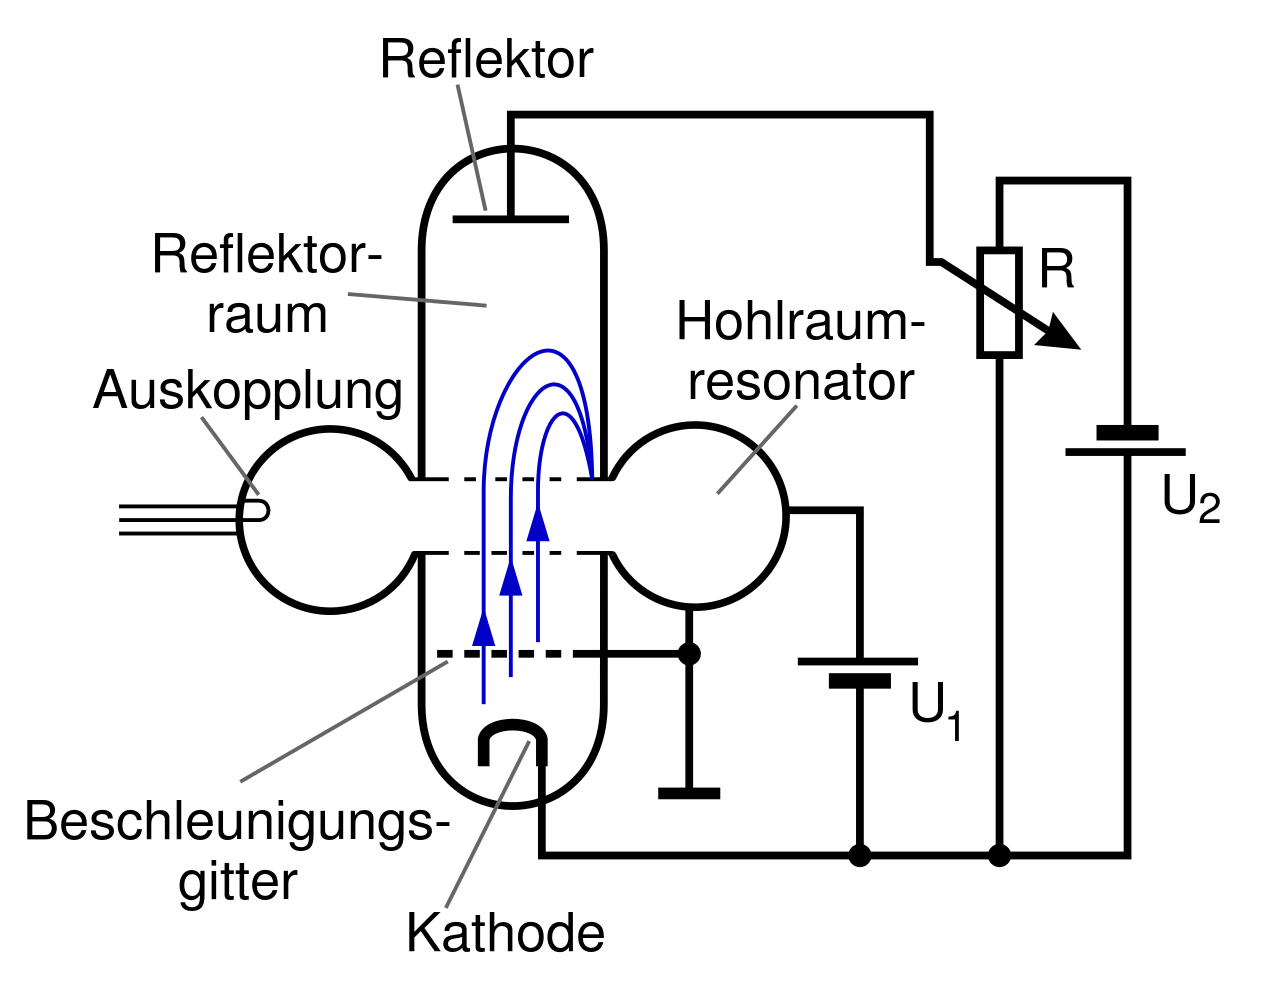
\includegraphics[width=6cm]{graphics/kly.png}
	\caption{Das Reflexklystron}
	\label{fig:kly}
\end{figure}
